\documentclass{article}
\usepackage[dblblindworkshop, nonatbib]{neurips_2026}
\workshoptitle{AI Foundations for Power Grids: From Models to Deployment at Scale (AI4PowerGrids Workshop @ NeurIPS 2026)}

\usepackage[utf8]{inputenc}
\usepackage[T1]{fontenc}
\usepackage{hyperref}
\usepackage{url}
\usepackage{booktabs}
\usepackage{amsfonts}
\usepackage{amsmath}
\usepackage{amssymb}
\usepackage{microtype}
\usepackage{graphicx}
\usepackage{float}
\usepackage{enumitem}

\setlength{\abovedisplayskip}{4pt}
\setlength{\belowdisplayskip}{4pt}
\setlength{\abovedisplayshortskip}{2pt}
\setlength{\belowdisplayshortskip}{2pt}
\setlength{\textfloatsep}{9pt plus 2pt minus 2pt}
\setlength{\parskip}{0pt}
\setlength{\parindent}{1em}

\newcommand{\pcc}{\mathrm{pcc}}
\newcommand{\zt}{\zeta}
\newcommand{\citep}[1]{\cite{#1}}
\newcommand{\todo}[1]{}

\title{Learning the Tie-Line Interface: GNN Fast Screening and Learned Local P/Q Control for Generation Interconnection}

\author{%
  Anonymous Author(s)\\  % Double-blind per the AI4PowerGrids CFP; de-anonymized at camera-ready.
}

\begin{document}

\maketitle

\begin{abstract}
Generation interconnection is an information problem: a planner must decide
how much power a new plant can inject through a single tie line without
breaking voltage stability or thermal limits on the bulk grid, and once
connected, the plant's smart inverters must keep the grid within limits using
only local measurements and one broadcast signal. We build both ends of that
loop on the IEEE 39-bus system with a dedicated gen-tie line, measured under
the full AC power-flow equations. A graph neural network screens injection
scenarios for congestion and stability headroom at $6.2$\% RMSE on max line
loading in distribution, with $91$\% congestion-decision accuracy against
$83$\% for a feature-based MLP, congestion-headroom ranking at Spearman
$0.75$, and $0.55$\,ms per scenario against $256$\,ms per AC solve. Under
an N-1 topology shift, all three surrogate models we test fail, with loading
errors of $28$\,--$32$\% RMSE: a measured, reported negative. A learned local
controller maps local PCC voltage, output, and the screening signal to an
active/reactive dispatch inside the plant's capability curve that, in the
closed loop, reduces the congestion-plus-voltage-plus-loss objective by
75\% over the IEEE 1547 volt-var baseline, with curtailment
concentrated in exactly the scenarios the GNN flags as congested. Failure
modes are reported on both ends, and every number regenerates from
committed artifacts.
\end{abstract}

%% =====================================================================
\section{Introduction}
%% =====================================================================

The interconnection queue is the front door of the energy transition: in the
United States, more than a terawatt of generation capacity is waiting to
connect, and the studies that decide whether a plant can connect check
thousands of candidate injections against the voltage and thermal limits of
the bulk transmission network \citep{gorman2025grid}. FERC Order 2023 was
written to make these studies fast enough to be re-run as the queue changes
\citep{ferc2023order}; ERCOT, which does not use FERC procedures, has the
same problem on the operating side, where plants behind weak tie lines get
curtailed because their real-time output congests the network
\citep{gorman2025grid,ercot2024reports}. Both are one information
problem: the boundary decision maker and the plant must know what the
plant's power does to the whole grid.

Two gaps stand between the queue and the control room. Screening: full AC
power flow is the gold standard, but a single solve takes tens of
milliseconds on a small system and seconds on a real one, and a queue study
runs thousands of them, while linearized DC screening is fast but blind to
voltage stability, the limit that binds on weak tie lines. Control: a
connected plant with smart inverters must regulate its active and reactive
output (P and Q) against grid conditions, and the standard today is a static
volt-var curve from IEEE 1547-2018 \citep{ieee1547}: a fixed function of
local voltage that neither sees grid congestion nor adapts to the plant's own
headroom.Learned local control exists on
distribution feeders \citep{cui2022lyapunov,guo2023rl,liu2025robust}, but a
controller is only as good as the signal it conditions on: a purely local
controller cannot know that a distant line is congested.

This paper builds the two ends of the loop and measures them together. The
first end is a graph neural network (GNN) that fast-screens injection
scenarios for a gen-tie: given the network state and a candidate plant
output, it predicts max line loading, minimum voltage, the loadability
margin $\lambda$ (voltage-stability headroom), and the congestion headroom
$\kappa$ (the plant-output multiplier before any line reaches 100\%
loading).GNNs are the established architecture because a power
network is a graph and injection effects propagate along edges \citep{donon2020graph,
falk2019warm,zhang2025risk}, evaluated for feasibility, constraint
violations, and out-of-distribution (OOD) shifts per this workshop's
standard. The second end is a learned local controller: a small policy maps
what the plant can measure locally (PCC voltage, its own real-time output)
plus one broadcast signal from the screening module (predicted max loading)
to a joint active/reactive dispatch, trained to imitate the grid-optimal
dispatch found by a dense AC scan. Every policy is evaluated with the full
AC power flow in the loop, since matching optimal setpoints in isolation
does not guarantee loop stability.

Two measured results carry the paper. The first is a screening result with
an honest negative: the GNN screens congestion decisions accurately in
distribution ($91$\% vs $83$\% for an MLP on the same features) and $470\times$
faster than one AC solve, but under an N-1 topology shift every surrogate
fails ($28$\,--$32$\% loading RMSE), which we report as a defined limit of
surrogate screening rather than a solved problem. The second is a positive
control result: the learned local controller reduces the
congestion-plus-voltage-plus-loss objective by 75\% over the IEEE
1547 baseline in the loop, keeping the improvement out of distribution.
Failure modes are reported on both ends.

%% =====================================================================
\section{Problem formulation}
%% =====================================================================

\subsection{AC power flow and the gen-tie model}
A transmission network is a set of buses $i\in\mathcal{B}$ connected by
lines and transformers. The AC power-flow equations balance net active and
reactive injection at every bus,
\begin{equation}
  P_i = \sum_j V_i V_j (G_{ij}\cos\theta_{ij} + B_{ij}\sin\theta_{ij}), \qquad
  Q_i = \sum_j V_i V_j (G_{ij}\sin\theta_{ij} - B_{ij}\cos\theta_{ij}),
  \label{eq:acpf}
\end{equation}
with $V_i$ the voltage magnitude, $\theta_{ij}=\theta_i-\theta_j$ the angle
difference, and $G_{ij},B_{ij}$ the conductance and susceptance of the line
between $i$ and $j$. A power-flow solution assigns voltages to every bus
given the injections $P_i,Q_i$; we solve \eqref{eq:acpf} with the full
Newton--Raphson solver of pandapower \citep{thurner2018pandapower}. A
scenario is \emph{feasible} if the equations have a real solution in
voltage limits; a non-converging AC solve, the practical signature of a
voltage collapse, is infeasible.

The generation tie (gen-tie) is a dedicated line from a plant bus $p$ to a
point of common coupling (PCC) bus $c$ on the bulk network. The plant is an
inverter-based resource with active output $P_g\in[0,P_{\max}]$ and reactive
output $Q_g$ constrained by its apparent-power rating
\begin{equation}
  Q_g^2 \le S_{\max}^2 - P_g^2,
  \label{eq:capability}
\end{equation}
so the available reactive headroom $Q_{\max}(P_g)=\sqrt{S_{\max}^2-P_g^2}$
shrinks as the plant produces more. Injecting $P_g$ through the tie line
changes every line flow and every voltage in the network; the screening
question is how much it changes them and how much headroom remains.

\subsection{Impact metrics}
For a scenario with plant output $P_g$ we compute four quantities under the
full AC equations: \emph{max line loading} $L_{\max}$ (largest line flow in
percent of rating; congested if $L_{\max}>100$); \emph{minimum voltage}
$V_{\min}$; the \emph{loadability margin} $\lambda$, the largest factor by
which loads and plant output can be scaled together before the AC power flow
loses a solution, minus one; and \emph{congestion headroom} $\kappa$, the
largest factor by which plant output alone can be raised before any line
reaches 100\% loading, both computed by bisection with a full AC solve at
every step.

\subsection{Information structure for local control}
The plant can measure its PCC voltage $V_{\pcc}$ and knows its own real-time
output $P_g$, but not the state of the bulk grid. We give it one additional
scalar, the screening signal $\zt$, the predicted max line loading from the
GNN screening module, modeling an operator that broadcasts a single
congestion indicator, as ERCOT-style curtailment signals already do
\citep{gorman2025grid}. The control problem is to choose the dispatch
$(P_g,Q_g)$ inside \eqref{eq:capability} as a function of
$(V_{\pcc},P_g,\zt)$ that keeps the grid inside its limits. The static
baseline is the IEEE 1547 volt-var curve, reactive output as a fixed
function of voltage with a $\pm 0.012$ pu deadband and full capability at
$|V_{\pcc}-1|=0.06$ \citep{ieee1547}; a second baseline holds a fixed 0.95
power factor.

%% =====================================================================
\section{Method}
%% =====================================================================

\subsection{End 1: GNN fast screening}
The network is a graph: buses are nodes, lines and transformers are edges.
Node features are per-bus active/reactive load and generation plus flags
for the slack, plant, and generator buses; edge features are resistance,
reactance, susceptance, rating, tap ratio, and a line-versus-transformer
indicator; scenario-level plant output and load regime are appended as two
extra node features. A three-layer graph isomorphism network (GIN)
\citep{xu2019gin} with edge-feature message passing and sum-pooling readout
predicts $L_{\max}, V_{\min}, \lambda$ and feasibility, trained with MSE
plus binary cross-entropy; $\kappa$ is predicted by a second instance on
the margin subset.

Training targets come exclusively from AC power-flow solves, so the model
inherits the full physics of \eqref{eq:acpf} rather than a linearized
approximation. Evaluation is constraint-aware: we report the accuracy of the
induced congestion decision ($L_{\max}>100$), Spearman rank correlation of
predicted versus true loadability margin, and end-to-end inference time
against the wall-clock time of one AC solve.

\subsection{End 2: learned local P/Q control}
The reference dispatch is computed per scenario by dense scan: we solve the
full AC power flow over a grid of $Q_g$ values inside \eqref{eq:capability}
and pick the reactive output minimizing the objective
\begin{equation}
  J(P_g,Q_g) = \max(0,L_{\max}-100)/100
  + \max(0,|V_{\pcc}-1|-0.012)/0.1
  + 0.5\,L_{\mathrm{loss}}/P_{\mathrm{load}},
  \label{eq:obj}
\end{equation}
whose terms penalize congestion, voltage deviation, and losses
($L_{\mathrm{loss}}$ is network loss, $P_{\mathrm{load}}$ total load). If the scenario is congested at the best reactive-only dispatch, we
repeat the scan over curtailment levels of active output and keep the
jointly optimal pair $(P^\star,Q^\star)$.

A small multilayer perceptron policy $\pi_\phi$ maps the local observation
$(V_{\pcc},P_g,\zt)$ to a reactive setpoint $Q$ and a curtailment ratio
$r\in[0.2,1]$, trained by regression against the oracle targets
$(Q^\star,P^\star/P_g)$. The policy is evaluated the way it would deploy:
the plant measures $V_{\pcc}$, the policy returns $(Q,r)$, the power flow is
re-solved, and the loop repeats to a fixed point, three iterations. This is
the system-level test: a controller that matched setpoints in isolation
could still fail here. The learned controller is compared against the IEEE
1547 volt-var curve and a fixed 0.95 power factor, both run in the same
closed loop, plus the oracle, on held-out scenarios and OOD load regimes.

%% =====================================================================
\section{Experiments}
%% =====================================================================

\subsection{Setup}
\label{sec:setup}
All experiments use the IEEE 39-bus (New England) test system
\citep{athay1979practical} from pandapower \citep{thurner2018pandapower},
augmented with a plant bus connected to bus 4 by a 15\,km, 230\,kV gen-tie
line rated at $S_{\max}=1000$ MVA with $P_{\max}=900$\,MW. Scenarios
randomize per-bus loads ($\pm15\%$ around a regime multiplier), redispatch
the nine conventional generators ($\pm10\%$), and draw the plant output
uniformly in $[0,900]$\,MW, at training load regimes
$\{0.85,1.0,1.15,1.30\}$ and OOD regimes $\{1.45,1.60\}$. The screening
dataset has 3{,}000 training scenarios plus 500 per OOD split (load regime
and an N-1 topology); margins are computed by bisection on a stratified
subset of 250 scenarios. The control dataset has 750 scenarios (150 OOD).
Every number regenerates from the repository scripts
(Appendix~\ref{app:repro}).

\begin{table}[t]
  \centering
  \small
  \begin{tabular}{lccc}
    \toprule
    & \multicolumn{3}{c}{max line loading RMSE (\%)} \\
    \cmidrule(lr){2-4}
    model & in-dist & OOD load & N-1 topo \\
    \midrule
    GNN & $6.2\pm0.3$ & $10.6\pm0.3$ & $31.3\pm1.8$ \\
    MLP & $11.0\pm0.4$ & $15.6\pm1.5$ & $28.0\pm2.3$ \\
    linear & $4.9\pm0.2$ & $9.2\pm0.0$ & $31.8\pm0.0$ \\
    \bottomrule
  \end{tabular}
  \caption{Mean over four seeds of max line loading RMSE (\%) for the GNN
  against an MLP and linear regression on the same node features, on the
  held-out training split, the OOD load regimes $\{1.45,1.60\}$, and the
  N-1 topology. The GNN beats the MLP in distribution and under the load
  shift, but no model generalizes to the topology shift, a failure reported
  in the body. Congestion decision accuracy is reported in the body.}
  \label{tab:screening}
\end{table}

\subsection{Result 1: the GNN screens injection scenarios accurately and cheaply}

We train the GNN on 2{,}400 of the 3{,}000 training scenarios and evaluate on
the held-out 600, the OOD load regimes, and the N-1 topology, over four
seeds. The headline number is the accuracy of the induced congestion
decision ($L_{\max}>100\%$): $91\%$ in distribution, against $83\%$ for an
MLP on the same node features (the linear model, given the regime
multiplier as an explicit feature, reaches $93\%$). Loading itself is
predicted with $6.2\pm0.3\%$ RMSE in distribution and $10.6\pm0.3\%$ under
the OOD load shift (Table~\ref{tab:screening}). End-to-end GNN screening of
a scenario takes $0.55$\,ms against $256$\,ms for one AC solve, a factor of
roughly $470$, which is what makes re-screening the queue feasible.

The shift that matters for interconnection is structural: a line trips and
the graph changes while the injections barely move. The N-1 split removes
the most heavily loaded line (buses 15--18, $77.9\%$ in the base case) and
re-solves every scenario on the modified network. This is the paper's
honest negative: no surrogate generalizes (Table~\ref{tab:screening}). The
GNN, fed the modified graph, reaches $31.3\%$ RMSE; the MLP and linear
baselines, fed node features that are statistically identical between the
two shifts, reach $28.0\%$ and $31.8\%$. The topology change moves the
loading distribution outside the training envelope and all three models
underpredict it; the failure holds for the graph-structured model too,
bounding what surrogate screening can promise without retraining.

Voltage-stability headroom is the harder target. On the 250 margin
scenarios (bisection over full AC solves), the GNN's congestion-headroom
prediction correlates with the true injection multiplier at Spearman
$\rho=0.75$ (n=200 pooled held-out points), ranking which injections are
closest to congesting the network. The loadability-margin prediction is
weaker, $\rho=0.31$: the model captures the broad trend of the margin
surface (Figure~\ref{fig:margin3d}) but not its sharp behavior near
collapse, so the signal we broadcast to the controller is the congestion
prediction.

\subsection{Result 2: the learned local controller beats the static curve in the loop}

Trained by regression against the dense-scan oracle on 600 scenarios, the
policy is evaluated in the closed loop on 120 held-out plus 150 OOD
scenarios, against the IEEE 1547 volt-var curve and the oracle, all in
the same loop (Table~\ref{tab:control}, Figure~\ref{fig:control}). On held-out scenarios the learned policy reaches a mean objective of
$J=0.079$ against $J=0.317$ for the volt-var droop, a reduction of
75\%, kept under the OOD load regimes ($J=0.605$ vs $0.846$ for no
control). The reduction comes from where the static curve is blind:
the droop reacts only to local voltage, while the learned policy
conditions on the broadcast screening signal $\zt$. It curtails real-time output in 43\% of held-out scenarios,
concentrated in the ones the screening module flags as congested
(Figure~\ref{fig:control}b). The dense
scan achieves $J=0.031$, so the learned policy closes 83\% of
the gap between the static baseline and the grid-optimal dispatch.

\subsection{Failure modes}
\label{sec:fail}

We report failures, not only means (Figure~\ref{fig:failures}). The
headline failure is structural: all three screening models degrade to
$28$\,--$32$\% loading RMSE under the N-1 topology shift (Result~1), so a
surrogate screener must be re-validated or retrained when the topology
changes, and flagged scenarios should defer to a full AC solve. The twelve
worst held-out errors are high-loading $1.30$-regime scenarios the model
underpredicts. The learned controller is worse than the static droop on
15\% of held-out scenarios, where the GNN underpredicts congestion
and the policy curtails less than it should; flagged cases get a human or
slower-solver review.%% =====================================================================
\section{Discussion and limitations}
%% =====================================================================
\enlargethispage{6\baselineskip}
The two results are two ends of one loop: the screening module broadcasts
\emph{one scalar}, predicted max line loading, and the plant's policy turns
that scalar plus its local voltage into an action that measurably reduces
congestion, voltage deviation, and losses.What this paper does not claim is stated plainly.
The 39-bus system with one gen-tie is a laboratory grid. The screening
signal is reliable for congestion, not yet for stability headroom
($\rho=0.31$); broadcasting it as a stability indicator would overclaim.
Surrogate screening does not generalize to the N-1 topology shift we
measure; generalizing without retraining remains open.The closed-loop controller is evaluated to a fixed point of the static
equations, not against transient dynamics.

%% =====================================================================
\section{Broader impact}
%% =====================================================================

The concrete pathway is the interconnection queue: a screener that runs in
milliseconds lets an operator re-run the study as the queue changes, and a
controller using a broadcast congestion signal lets a connected plant
manage output against real-time conditions.
The honest stage matters as much: this is a 39-bus laboratory result, not
authorization to deploy learned control on a live system, and the
deployment envelope is exactly the failure modes we report
(Section~\ref{sec:fail}): flag-and-defer for the screening tail, with a
fallback to the static curve when the signal is unreliable.

%% LLM disclosure required by the workshop CFP, before references.
\vspace{-0.7em}
\section*{Use of generative AI}
The manuscript was drafted with the assistance of a large language model;
all experiments, code, and figures were produced by the authors' own
pipeline, per the AI4PowerGrids call for papers.

%% =====================================================================
\bibliographystyle{plainnat}
%% =====================================================================
\begin{thebibliography}{99}
\small

\bibitem[Athay et~al.(1979)]{athay1979practical}
Athay, T., Podmore, R., and Virmani, S.
\newblock A practical method for the direct analysis of transient stability.
\newblock {\em IEEE Trans. Power Appar. Syst.}, PAS-98:573--584, 1979.

\bibitem[Cui and Zhang(2022)]{cui2022lyapunov}
Cui, W. and Zhang, B.
\newblock Lyapunov-regularized reinforcement learning for power system
  transient stability.
\newblock {\em IEEE Control Systems Letters}, 6:974--979, 2022.

\bibitem[Donon et~al.(2020)]{donon2020graph}
Donon, B., Cl\'ement, R., Donnot, B., Marot, A., Guyon, I., and
  Schoenauer, M.
\newblock Neural networks for power flow: graph neural solver.
\newblock {\em Electric Power Systems Research}, 189:106547, 2020.

\bibitem[Falk et~al.(2019)]{falk2019warm}
Falk, T., Donon, B., Guyon, I., Donnot, B., and Schoenauer, M.
\newblock Warm-starting AC optimal power flow with graph neural networks.
\newblock In {\em NeurIPS 2019 Workshop on Tackling Climate Change with
  Machine Learning}, 2019.

\bibitem[FERC(2023)]{ferc2023order}
Federal Energy Regulatory Commission.
\newblock Improvements to generator interconnection procedures and
  agreements.
\newblock {\em Order No. 2023}, Docket RM22-14-000, 2023.

\bibitem[ERCOT(2024)]{ercot2024reports}
Electric Reliability Council of Texas.
\newblock 2023 state of the grid report.
\newblock ERCOT, 2024.

\bibitem[Gorman et~al.(2025)]{gorman2025grid}
Gorman, W., et al.
\newblock Grid connection barriers to renewable energy deployment.
\newblock {\em Joule}, 9(2):101803, 2025.

\bibitem[Guo and Lei(2023)]{guo2023rl}
Guo, Y. and Lei, Q.
\newblock Reinforcement learning-based smart inverter control with polar
  action space.
\newblock {\em IEEE Trans. Power Systems}, 38(4), 2023.

\bibitem[IEEE(2018)]{ieee1547}
IEEE.
\newblock IEEE Standard for Interconnection and Interoperability of
  Distributed Energy Resources with Associated Electric Power Systems
  Interfaces.
\newblock {\em IEEE Std 1547-2018}, 2018.

\bibitem[Liu et~al.(2025)]{liu2025robust}
Liu, Y., Guo, Y., and Xu, T.
\newblock Robust deep reinforcement learning for inverter-based volt-var
  control in partially observable distribution networks.
\newblock {\em Applied Energy}, 2025.

\bibitem[Marot et~al.(2021)]{marot2021l2rpn}
Marot, A., Donnot, B., Chaouache, K., Kelly, A., Dulac-Arnold, C., et al.
\newblock Learning to run a power network challenge for training topology
  controllers.
\newblock {\em Electric Power Systems Research}, 2021.

\bibitem[Okoyomon et~al.(2025)]{okoyomon2025gnn}
Okoyomon, E., et al.
\newblock A framework for assessing the generalizability of GNN-based power
  flow solvers.
\newblock In {\em e-Energy 2025}, ACM, 2025.

\bibitem[Thurner et~al.(2018)]{thurner2018pandapower}
Thurner, L., et al.
\newblock pandapower: an open-source python tool for convenient modeling,
  analysis, and optimization of electric power systems.
\newblock {\em IEEE Trans. Power Systems}, 33(6):6510--6521, 2018.

\bibitem[Xu et~al.(2019)]{xu2019gin}
Xu, K., Hu, W., Leskovec, J., and Jegelka, S.
\newblock How powerful are graph neural networks?
\newblock In {\em International Conference on Learning Representations},
  2019.

\bibitem[Zhang et~al.(2025)]{zhang2025risk}
Zhang, Y., et al.
\newblock Operational risk quantification of power grids using graph neural
  networks.
\newblock {\em Energy and AI}, 2025.

\bibitem[Zhou et~al.(2024)]{powergraph2024}
Zhou, X., et al.
\newblock A power grid benchmark dataset for graph neural networks.
\newblock In {\em Advances in Neural Information Processing Systems
  Datasets and Benchmarks Track}, 2024.

\end{thebibliography}

%% =====================================================================
\appendix
\section{Reproduction statement}
\label{app:repro}
%% =====================================================================

Every number in this paper is regenerated from committed artifacts in the
project repository: the scenario generator
(\texttt{experiments/make\_screening\_data.py},
\texttt{experiments/make\_control\_data.py}), the trainers
(\texttt{experiments/train\_screening.py},
\texttt{experiments/train\_control.py}), and the figure script
(\texttt{experiments/generate\_figures.py}). The data files and per-seed
result JSONs are committed. All power-flow quantities come from pandapower
AC solves; the loadability and congestion margins are bisection results over
full AC solves; the control oracle is a dense scan over the reactive
capability curve with full AC solves; the baselines are run in the closed
loop to a fixed point. The plant is modeled as a constant-voltage resource
in the screening study (a plant holding its terminal voltage) and as a PQ
injection in the control study, where reactive dispatch is the control
variable; a generator with a fixed voltage setpoint would ignore the
reactive schedule entirely. Compute is a single CPU workstation; typical
wall time for the full pipeline is a few hours.

\section{Additional figures and tables}
%% =====================================================================

\begin{figure}[ht]
  \centering
  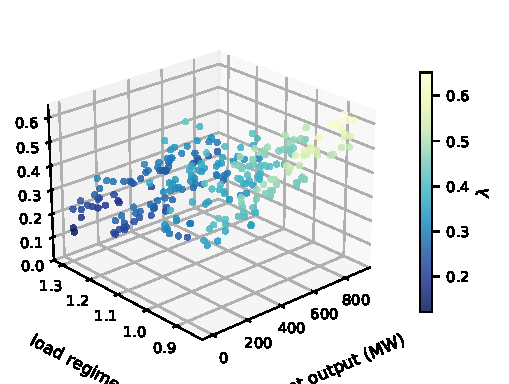
\includegraphics[width=0.72\textwidth]{figures/fig2_margin3d.pdf}
  \caption{Loadability margin $\lambda$ over the plant output and the load
  regime (250 scenarios, exact bisection over full AC power flow). The
  margin falls as the plant output rises and as the load regime rises;
  the surface is smooth in both directions, which is what lets the GNN
  regress it from a modest number of scenarios.}
  \label{fig:margin3d}
\end{figure}

\begin{figure}[ht]
  \centering
  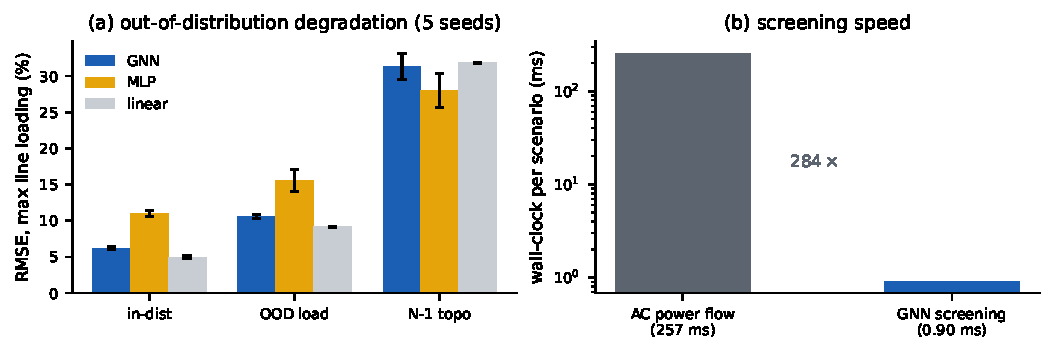
\includegraphics[width=0.95\textwidth]{figures/fig4_ood_speed.pdf}
  \caption{Left: per-split max line loading RMSE for the GNN, the MLP, and
  linear regression (mean and standard deviation over four seeds); the GNN
  beats the MLP in distribution and under the load shift, and all three
  models degrade to $28$\,--$32$\% under the N-1 topology shift. Right:
  wall-clock time per scenario for one full AC power-flow solve against
  end-to-end GNN screening inference (four-seed mean; log scale).}
  \label{fig:ood}
\end{figure}

\begin{figure}[ht]
  \centering
  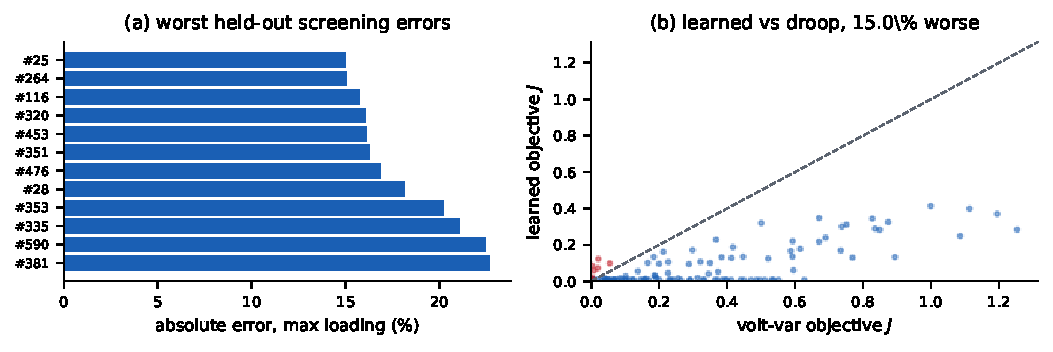
\includegraphics[width=0.95\textwidth]{figures/fig5_failures.pdf}
  \caption{Left: the twelve worst held-out screening errors, the scenarios
  where the surrogate is least reliable and where a human review step
  should be triggered. Right: closed-loop objective of the learned
  controller against the IEEE 1547 volt-var baseline per held-out
  scenario, with the scenarios where the learned controller is worse shown
  in red.}
  \label{fig:failures}
\end{figure}

\subsection{Screening performance}

\begin{figure}[ht]
  \centering
  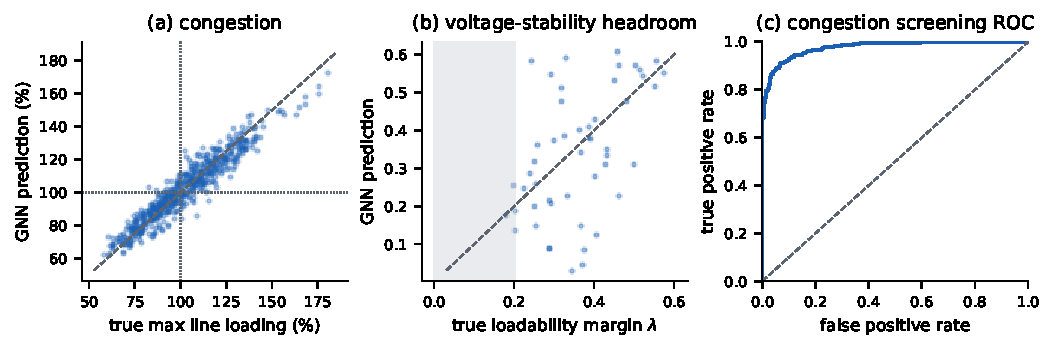
\includegraphics[width=0.95\textwidth]{figures/fig1_screening.pdf}
  \caption{Screening performance of the GNN on held-out scenarios
  (n=600, 4 seeds) under the full AC power flow. Left: predicted versus
  true max line loading; the 45-degree line is exact prediction, points
  above 100\% on both axes are congested scenarios. Middle: predicted versus
  true loadability margin, with the near-collapse region ($\lambda<0.2$)
  shown; Spearman rank correlation reported in the body. Right: congestion
  screening ROC (any line above 100\% loading) with the random baseline.
  Baselines: an MLP on the same node features and linear regression
  (Table~\ref{tab:screening}).}
  \label{fig:screening}
\end{figure}

\subsection{Closed-loop control results}

\begin{figure}[ht]
  \centering
  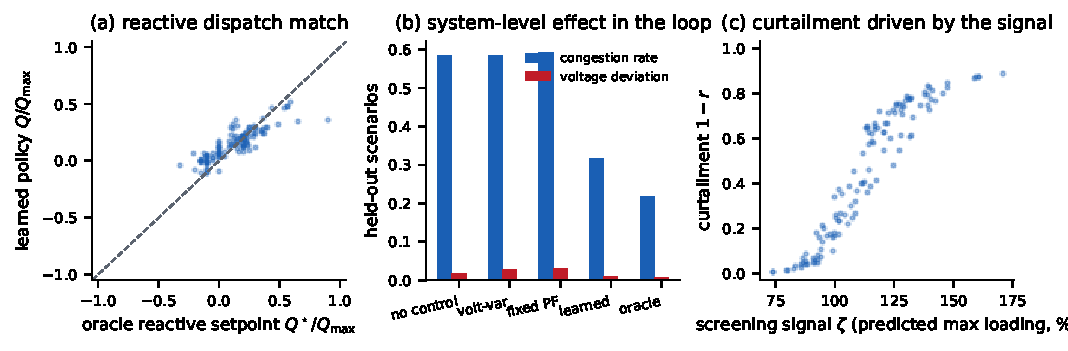
\includegraphics[width=0.95\textwidth]{figures/fig3_control.pdf}
  \caption{Closed-loop control results on held-out scenarios (n=120,
  seed 0). Left: reactive setpoint applied by the learned policy in
  the closed loop against the dense-scan oracle setpoint, both normalized
  by the plant's reactive headroom; agreement is good where headroom
  exists. Middle: congestion rate and mean voltage deviation under no
  control, the IEEE 1547 volt-var droop, fixed 0.95 power factor, the
  learned policy, and the oracle, all run inside the AC power flow to a
  fixed point. Right: curtailment $1-r$ applied by the learned policy
  against the screening signal $\zt$; curtailment concentrates in the
  scenarios the GNN flags as congested.}
  \label{fig:control}
\end{figure}

\begin{table}[ht]
  \centering
  \small
  \begin{tabular}{lcccc}
    \toprule
    & \multicolumn{2}{c}{held-out} & \multicolumn{2}{c}{OOD load} \\
    \cmidrule(lr){2-3}\cmidrule(lr){4-5}
    policy & objective $J$ & congestion (\%) & objective $J$ & congestion (\%) \\
    \midrule
    no control & 0.193 & 58 & 0.846 & 97 \\
    IEEE 1547 volt-var & 0.317 & 58 & 1.652 & 100 \\
    fixed 0.95 PF & 0.355 & 59 & 1.157 & 97 \\
    learned policy & 0.079 & 31 & 0.605 & 98 \\
    oracle (dense scan) & 0.031 & 22 & 0.199 & 90 \\
    \bottomrule
  \end{tabular}
  \caption{Mean objective \eqref{eq:obj} and congestion rate under each
  policy on the held-out split of the control scenarios and on the OOD
  load regimes. The learned policy is evaluated in the closed loop to a
  fixed point, the same loop in which the baselines and the dense-scan
  oracle are evaluated. The oracle is the per-scenario optimum of the
  dense scan, so it is the achievable upper bound.}
  \label{tab:control}
\end{table}

\subsection{Per-seed screening results}
All screening numbers are means over seeds; the per-seed values below are
reported for completeness. Congestion decision accuracy is the fraction of
scenarios where the model's predicted max loading is on the correct side of
the $100\%$ threshold.

\begin{table}[ht]
  \centering
  \small
  \begin{tabular}{lccc|ccc}
    \toprule
    & \multicolumn{3}{c}{max loading RMSE (\%)} & \multicolumn{3}{c}{congestion acc} \\
    \cmidrule(lr){2-4}\cmidrule(lr){5-7}
    seed & in-dist & OOD load & N-1 topo & in-dist & OOD load & N-1 topo \\
    \midrule
    0 & 6.42 & 10.14 & 28.29 & 0.913 & 0.992 & 0.984 \\
    1 & 6.20 & 10.62 & 32.59 & 0.908 & 0.990 & 0.984 \\
    2 & 6.45 & 10.74 & 31.49 & 0.923 & 0.994 & 0.986 \\
    3 & 5.83 & 10.92 & 32.83 & 0.912 & 0.994 & 0.984 \\
    \bottomrule
  \end{tabular}
  \caption{Per-seed GNN screening metrics, showing the variance across
  seeds that the body reports as means.}
  \label{tab:perseed_screen}
\end{table}

\subsection{Per-seed control results}

\begin{table}[ht]
  \centering
  \small
  \begin{tabular}{lcccc}
    \toprule
    seed & held-out $J$ & OOD $J$ & held-out cong (\%) & OOD cong (\%) \\
    \midrule
    0 & 0.073 & 0.594 & 32 & 98 \\
    1 & 0.094 & 0.617 & 33 & 98 \\
    2 & 0.073 & 0.603 & 31 & 98 \\
    3 & 0.065 & 0.596 & 24 & 98 \\
    4 & 0.091 & 0.617 & 33 & 98 \\
    \bottomrule
  \end{tabular}
  \caption{Per-seed closed-loop control metrics for the learned policy.}
  \label{tab:perseed_ctrl}
\end{table}

\subsection{Training details}
The screening GNN has three GIN layers of width 96 with edge-feature
message passing (GINE), sum-pooling readout, and a three-output head
(max loading, min voltage, feasibility logit); a second instance with a
three-output head on the margin subset predicts loadability margin,
congestion headroom, and feasibility. It is trained for 70 epochs (50 for
the margin head) with Adam at learning rate $3\times10^{-3}$, cosine decay,
weight decay $10^{-5}$, and batch size 256, on MSE plus binary
cross-entropy. The MLP baseline is two hidden layers of width 96 on the
same flattened and normalized node features with the same optimizer. The
linear baseline is ordinary least squares on the same features. The control
policy is a two-hidden-layer MLP (width 64) mapping
$(V_{\pcc}, P_g, \zt)$ to a normalized reactive setpoint (tanh, rescaled by
the capability curve) and a curtailment ratio (sigmoid, rescaled to
$[0.2,1]$), trained for 200 epochs with Adam at $10^{-3}$, batch 128, MSE
regression against the dense-scan oracle targets. The closed-loop
controller and all baselines are iterated to a fixed point with three full
AC solves. All models run on CPU; the scenario generators use eight
multiprocessing workers.

%% =====================================================================
%% Domain evaluation checklist (required by the AI4PowerGrids CFP; does not
%% count toward the 4-page main-text limit).
%% =====================================================================
\section*{Domain evaluation checklist}

\begin{enumerate}[leftmargin=1.4em,itemsep=2pt,topsep=2pt]
  \item \textbf{Physics feasibility.} All training targets, the control
  oracle, and every closed-loop evaluation come from full Newton--Raphson
  AC power-flow solves (pandapower), never a linearized approximation.
  Constraint statistics are reported, not only aggregate error: congestion
  is defined by the induced decision accuracy on $L_{\max}>100\%$ (body,
  Result~1 and Table~1) and voltage deviation by the exact margin
  violation rate in the control loop (Result~2).
  \item \textbf{Out-of-distribution evaluation.} Both components are
  evaluated on two distribution shifts not seen in training: load regimes
  at multipliers $\{1.45,1.60\}$ above the training range $\{0.85,1.30\}$,
  and an N-1 topology with the most heavily loaded line removed. The
  screening models' degradation on the N-1 shift is reported as a primary
  failure mode (Section~\ref{sec:setup}, Results~1--2, Figure~\ref{fig:ood}).
  \item \textbf{Failure modes.} Reported alongside aggregate metrics:
  worst-case screening errors and the scenarios where the learned
  controller underperforms the static volt-var baseline
  (Section~\ref{sec:fail}, Figure~\ref{fig:failures}).
  \item \textbf{System-level effect.} The learned controller is not scored
  on setpoint error. It is placed inside the AC power flow and run to a
  fixed point, and the downstream quantities (congestion rate, voltage
  deviation, losses, curtailment) are reported against baselines run in
  the same loop (Result~2).
  \item \textbf{Data and code.} The full pipeline (scenario generators,
  trainers, figure script) and the generated data and per-seed result
  files will be released under a permissive license at an anonymous link
  at submission; no proprietary data is used.
\end{enumerate}

\end{document}
